\documentclass[spanish]{beamer}
\usepackage[ansinew]{inputenc} % Acepta caracteres en castellano
\usepackage[spanish]{babel}    % silabea palabras castellanas
\usepackage{amsmath}
\usepackage{mathtools,cancel} % cancela con una flecha \cancelto{0}{XXXX}
\renewcommand{\CancelColor}{\color{red}} %change cancel color to red
\usepackage{amsfonts}
\usepackage{amssymb}
\usepackage{dsfont}
\usepackage{graphicx}
\usepackage{geometry}
\usetheme{Madrid}
\usecolortheme{beaver}
\usepackage{textpos}
% Logo  en el comienzo 
\addtobeamertemplate{frametitle}{}{%
\begin{textblock*}{100mm}(.85\textwidth,-1cm)
{\includegraphics[height=0.4in, keepaspectratio=true]{/Users/luisnunez/Dropbox/MisDocumentos/UIS/UISImagenInstitucional/UISLOGO.png}}
\end{textblock*}}

\begin{document}

\title{\textbf{Par�ntesis de Poisson} }
\author[L.A. N��ez]{\textbf{Luis A. N��ez}}  
\institute[UIS]{\textit{Escuela de F�sica, Facultad de Ciencias, } \\
\textit{Universidad Industrial de Santander, Santander, Colombia } \\
{\includegraphics[height=0.4in, keepaspectratio=true]{/Users/luisnunez/Dropbox/MisDocumentos/UIS/UISImagenInstitucional/UISLOGO.png}}
}
\date{\today}
\maketitle


\begin{frame}
\frametitle{Agenda}
  \tableofcontents
\end{frame}
%
%%%%% Diapo 2
\subsection{Definici�n}
\frame{
\frametitle{Par�ntesis de Poisson: Definici�n}
\begin{itemize}  
	\item<1-> Sea una funci�n $f\left(q_i, p_i, t\right)$ en el espacio de fase $\left(q_i, p_i\right)$, $i=1, \ldots, s$, de un sistema mec�nico con un Hamiltoniano $\mathcal{H}\left(q_i, p_i, t\right)$.
	\item<2-> La derivada total de $f$ es $\frac{d f}{d t}=\sum_{i=1}^s\left(\frac{\partial f}{\partial q_i} \dot{q}_i+\frac{\partial f}{\partial p_i} \dot{p}_i\right)+\frac{\partial f}{\partial t}$.
	\item<3-> Sus ecuaciones de Hamilton son $\dot{q}_i=\frac{\partial \mathcal{H}}{\partial p_i}, \quad \dot{p}_i=-\frac{\partial \mathcal{H}}{\partial q_i}$
	\item<4-> Sustituyendo, tenemos $\frac{d f}{d t}=\sum_{i=1}^s\left(\frac{\partial f}{\partial q_i} \frac{\partial \mathcal{H}}{\partial p_i}-\frac{\partial f}{\partial p_i} \frac{\partial \mathcal{H}}{\partial q_i}\right)+\frac{\partial f}{\partial t}$
	\item<5-> Entonces el par�ntesis de Poisson de la funci�n $f$ para un sistema con hamiltoniano $\mathcal{H}$ es $\{f, \mathcal{H}\} \equiv \sum_{i=1}^s\left(\frac{\partial f}{\partial q_i} \frac{\partial \mathcal{H}}{\partial p_i}-\frac{\partial f}{\partial p_i} \frac{\partial \mathcal{H}}{\partial q_i}\right)$.
	\item<6-> Con lo cual $\frac{d f}{d t}=\{f, \mathcal{H}\}+\frac{\partial f}{\partial t} $
	\item<7-> Si $f$ no depende expl�citamente del tiempo (cantidad conservada), tenemos $\{f, \mathcal{H}\}=0$
	\item<8-> Para $f\left(q_i, p_i, t\right)$ y $g\left(q_i, p_i, t\right)$ podemos definir el par�ntesis de Poisson de ${f}$ y $g$ como $\{f, g\} \equiv \sum_{i=1}^s\left(\frac{\partial f}{\partial q_i} \frac{\partial g}{\partial p_i}-\frac{\partial f}{\partial p_i} \frac{\partial g}{\partial q_i}\right) .$
\end{itemize}
}
%
%%%%% Diapo 2
\subsection{Propiedades}
\frame{
\frametitle{Par�ntesis de Poisson: Propiedades 1/2}
\begin{itemize}  
	\item<1-> El par�ntesis de Poisson puede ser considerado como una operaci�n entre dos funciones definidas en un espacio algebraico que asigna otra funci�n en ese espacio.
	\item<2-> El par�ntesis de Poisson, como operaci�n algebraica, posee las siguientes propiedades (caracter�sticas de lo que se denomina �lgebra de Lie):
	\begin{itemize}
		\item $\{f, g\}=-\{g, f\}, \quad\{f, f\}=0 \quad$ (antisimetr�a).
		\item $\{f, c\}=0, \quad$ si $c=$ cte.
		\item $\left\{a f_1+b f_2, g\right\}=a\left\{f_1, g\right\}+b\left\{f_2, g\right\}, \quad a, b=$ ctes, un operador lineal.
		\item $\left\{f_1 f_2, g\right\}=f_1\left\{f_2, g\right\}+f_2\left\{f_1, g\right\}, \quad$ (no asociativo).
		\item $\{f,\{g, \mathcal{H}\}\}+\{g,\{h, f\}\}+\{h,\{f, g\}\}=0 \quad$  la identidad de Jacobi.
	\end{itemize}
\end{itemize}
}
%
%
%\section{Secci�n}
\frame{
\frametitle{Par�ntesis de Poisson: Propiedades 2/2}
\begin{itemize}  
	\item<1-> Como $p_i$ y $q_i$ representan coordenadas independientes tenemos $\left\{q_i, f\right\}=\sum_{k=1}^s\left(\frac{\partial q_i}{\partial q_k} \frac{\partial f}{\partial p_k}-
	\cancelto{0}{\frac{\partial q_k}{ \partial p_k}} \frac{\partial f}{\partial q_k}\right)=\sum_{k=1}^s \delta_{i k} \frac{\partial f}{\partial p_k}=\frac{\partial f}{\partial p_i}$ 
	$\left\{p_i, f\right\}=\sum_{k=1}^s \left(\cancelto{0} {\frac{\partial p^{\prime}}{ \partial q_k}} \frac{\partial f}{\partial p_k}-\frac{\partial p_i}{\partial p_k} \frac{\partial f}{\partial q_k}\right)=-\sum_{k=1}^s \delta_{i k} \frac{\partial f}{\partial q_k}=-\frac{\partial f}{\partial q_i} .$
	\item<2-> Si $f=p_j$, � $f=q_j$, $\left\{q_i, q_j\right\}=0, \quad\left\{p_i, p_j\right\}=0, \quad\left\{q_i, p_j\right\}=\delta_{i j}$
	\item<3-> Utilizando par�ntesis de Poisson, las ecuaciones de Hamilton pueden escribirse como 
	$\dot{q}_i  =\frac{\partial \mathcal{H}}{\partial p_i}=\left\{q_i, \mathcal{H}\right\} \quad \dot{p}_i  =-\frac{\partial \mathcal{H}}{\partial q_i}=\left\{p_i, \mathcal{H}\right\}$
	\item<4-> En Mec�nica Cu�ntica, la operaci�n $[A, B]=A B-B A$ se denomina el conmutador de los operadores u observables $A$ y $B$.
	\item<5-> La estructura algebraica de la Mec�nica Cl�sica, expresada en las propiedades de los par�ntesis de Poisson, se preserva en la Mec�nica Cu�ntica. En particular, $\left\{q_i, p_j\right\}=i \hbar \delta_{i j}$, donde $\hbar$ es la constante de Planck (dividida por $2 \pi)$.
\end{itemize}
}
%
%%%%% Diapo 2
\subsection{Dos ejemplos}
\frame{
\frametitle{Dos Ejemplos}
\begin{itemize}  
	\item<1-> Calcular $\{r, \mathbf{p}\}$, donde $r=\left(x^2+y^2+z^2\right)^{1 / 2}$
	\begin{itemize}
		\item $\{r, \mathbf{p}\}=\left\{r, p_x\right\} \hat{\mathbf{x}}+\left\{r, p_y\right\} \hat{\mathbf{y}}+\left\{r, p_z\right\} \hat{\mathbf{z}}$
		\item $\left\{r, p_x\right\}=\sum_{i=1}^3\left(\frac{\partial r}{\partial q_i} \frac{\partial p_x}{\partial p_i}-\frac{\partial r}{\partial p_i} \frac{\partial p_x}{\partial q_i}\right)=\frac{\partial r}{\partial x} \frac{\partial p_x}{\partial p_x}=\frac{x}{r}$
		\item $\left\{r, p_y\right\}=\frac{y}{r}, \quad\left\{r, p_z\right\}=\frac{z}{r}$
		\item luego $\{r, \mathbf{p}\}=\frac{x}{r} \hat{\mathbf{x}}+\frac{y}{r} \hat{\mathbf{y}}+\frac{z}{r} \hat{\mathbf{z}}=\frac{\mathbf{r}}{r}=\hat{\mathbf{r}} $
	\end{itemize}
	\item<2->  Dadas las componentes del momento angular $\mathbf{L}=\mathbf{r} \times \mathbf{p}$:
	$L_x=y p_z-z p_y, \quad L_y=z p_x-x p_z, \quad L_z=x p_y-y p_x$ \\
	Calcular los par�ntesis de Poisson para las componentes de {\bf p} y {\bf L}: \\ 	
	$\left\{p_y, L_x\right\}=-\frac{\partial L_x}{\partial y}=-p_z$;  $\quad \left\{p_x, L_x\right\}=-\frac{\partial L_x}{\partial x}=0$; $\quad \left\{p_z, L_y\right\}=-\frac{\partial L_y}{\partial z}=-p_x$ \\
 $\left\{L_x, L_y\right\} =\sum_{i=1}^3\left(\frac{\partial L_x}{\partial q_i} \frac{\partial L_y}{\partial p_i}-\frac{\partial L_x}{\partial p_i} \frac{\partial L_y}{\partial q_i}\right)$ \\$ 
		\left\{L_x, L_y\right\} = \left(\frac{\partial L_x}{\partial x} \frac{\partial L_y}{\partial p_x}-\frac{\partial L_x}{\partial p_x} \frac{\partial L_y}{\partial x}\right)+\left(\frac{\partial L_x}{\partial y} \frac{\partial L_y}{\partial p_y}-\frac{\partial L_x}{\partial p_y} \frac{\partial L_y}{\partial y}\right)+\left(\frac{\partial L_x}{\partial z} \frac{\partial L_y}{\partial p_z}-\frac{\partial L_x}{\partial p_z} \frac{\partial L_y}{\partial z}\right)$ \\
	$\left\{L_x, L_y\right\} =x p_y-y p_x=L_z$; $\quad \left\{L_y, L_z\right\}  =L_x$ $\quad \left\{L_z, L_x\right\}  =L_y$
	\item<3-> 	En general, $\left\{L_i, L_j\right\}=\epsilon_{i j k} L_k$. En Mec�nica Cu�ntica,  $\left[L_i, L_j\right]=i \hbar \epsilon_{i j k} L_k$.	
\end{itemize}
}
%
%%%%% Diapo 2
\subsection{Par�ntesis de Poisson y Transformaciones Can�nicas}
\frame{
\frametitle{Par�ntesis de Poisson y Transformaciones}
\begin{itemize}  
	\item<1-> 
\end{itemize}
}
 
\end{document}
%
%%%%% Diapo 2
\section{Secci�n}
\frame{
\frametitle{T�tulo transparencia}
\begin{itemize}  
	\item<1-> 
\end{itemize}
}
	\begin{figure}[t]
		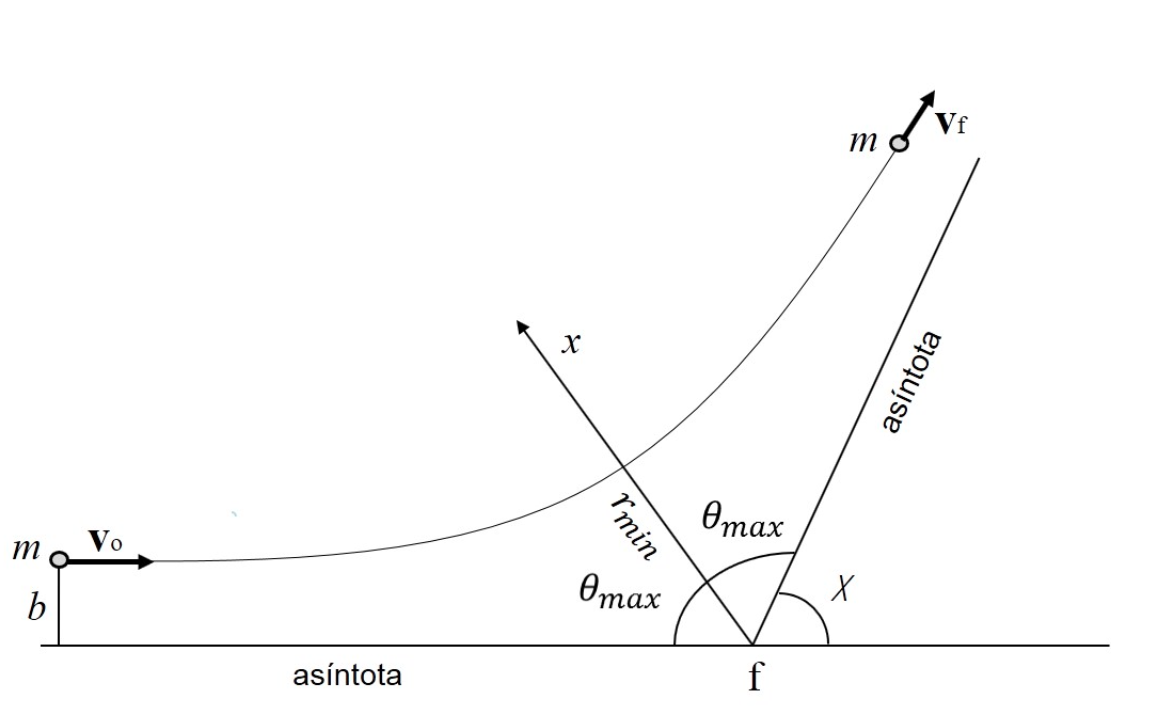
\includegraphics[width=1.8in]{Figuras/Dispersion.png}
   	\end{figure}
%
%%%%% Diapo 2
\section{Secci�n}
\frame{
\frametitle{T�tulo transparencia}
Las funciones generadores pueden no depender de todas las variables $\left(q_i, p_i, Q_i, P_i, t\right)$ y 
 $\frac{d  \mathcal{F}}{d t}=\sum_{i=1}^s p_i \dot{q}_i-\sum_{i=1}^s P_i \dot{Q}_i+\left(\tilde{\mathcal{H}}-\mathcal{H}\right)$ nos permite identificar varias 
\begin{itemize}
	\item<1-> La funci�n $\mathcal{F}_1\left(q_i, Q_i, t\right)$ genera  $p_i=p_i(q, Q, t), P_i=P_i(q, Q, t)$  
	\item<1-> $\mathcal{F}_1=\mathcal{F}_1\left(q_i, Q_i, t\right) \Rightarrow \frac{d \mathcal{F}_1}{d t}=\sum_{i=1}^s\left(\frac{\partial \mathcal{F}_1}{\partial q_i} \dot{q}_i+\frac{\partial \mathcal{F}_1}{\partial Q_i} \dot{Q}_i\right)+\frac{\partial \mathcal{F}_1}{\partial t}$.
	\item<1-> $p_i=\frac{\partial \mathcal{F}_1}{\partial q_i} =p_i(q, Q, t); \quad P_i=-\frac{\partial \mathcal{F}_1}{\partial Q_i} =P_i(q, Q, t); \quad \tilde{\mathcal{H}} =\mathcal{H}+\frac{\partial \mathcal{F}_1}{\partial t}$
\end{itemize}
}	
